\documentclass[tikz]{standalone}

\usetikzlibrary{positioning}

\begin{document}
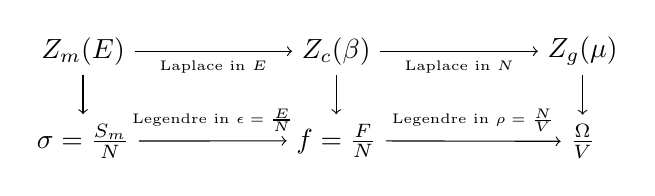
\begin{tikzpicture}[trafo/.style={midway,font=\tiny}]

  \def\hd{2}\def\vd{0.5}

  \node (Zm) at (0,0) {$Z_m(E)$};
  \node[right=\hd of Zm] (Zc) {$Z_c(\beta)$};
  \node[right=\hd of Zc] (Zg) {$Z_g(\mu)$};

  \node[below=\vd of Zm] (Sm) {$\sigma = \frac{S_m}{N}$};
  \node[below=\vd of Zc] (F) {$f = \frac{F}{N}$};
  \node[below=\vd of Zg] (O) {$\frac{\Omega}{V}$};

  \draw[->] (Zm) -- (Sm);
  \draw[->] (Zc) -- (F);
  \draw[->] (Zg) -- (O);

  \draw[->] (Zm) -- (Zc) node[trafo,below] {Laplace in $E$};
  \draw[->] (Zc) -- (Zg) node[trafo,below] {Laplace in $N$};

  \draw[->] (Sm) -- (F) node[trafo,above] {Legendre in $\epsilon = \frac{E}{N}$};
  \draw[->] (F) -- (O) node[trafo,above] {Legendre in $\rho = \frac{N}{V}$};

\end{tikzpicture}
\end{document}
